\section{Regressão de Poisson}

\subsection{Leituras Recomendadas}
\begin{frame}{Regressão de Poisson - Leituras Recomendadas}
	\begin{vfilleditems}
		\item \textcite{gelman2013bayesian} - Capítulo 16: Generalized linear models
		\item \textcite{mcelreath2020statistical}:
		\begin{vfilleditems}
			\item Capítulo 10: Big Entropy and the Generalized Linear Model
			\item Capítulo 11, Seção 11.2: Poisson regression
		\end{vfilleditems}
		\item \textcite{gelman2020regression} - Capítulo 15, Seção 15.2: Poisson and negative binomial regression
		\item \textcite{storopoli2021estatisticabayesianaR} - Regressão de Poisson
		\item Tutorial de \texttt{rstanarm} de \textcite{muth2018user}
		\item \href{http://mc-stan.org/rstanarm/articles/count.html}{Vinheta do \texttt{rstanarm} sobre Modelos Lineares Generalizados com dados de Contagem}
	\end{vfilleditems}
\end{frame}

\begin{frame}{Bem-Vindo ao Mundo Mágico dos Modelos Lineares Generalizados}
	Saindo do universo dos modelos lineares, começamos a nos aventurar nos modelos
	linares generalizados (\textit{generalized linear models} -- GLM).
	\vfill
	O segundo deles é a \textbf{regressão de Poisson}.
\end{frame}

\subsection{Dados de Contagem\footnote{\textit{count data}}}
\begin{frame}{Dados de Contagem}
	Regressão de Poisson é usada quando a nossa variável dependente só pode
	tomar \textbf{valores positivos}, geralmente em contextos de
	\textbf{dados de contagem}.
\end{frame}

\subsection{O que é Regressão de Poisson?}
\begin{frame}{O que é Regressão de Poisson?}
	Uma regressão de Poisson se comporta exatamente como um modelo linear:
	faz uma predição simplesmente computando uma soma ponderada das variáveis
	independentes $\mathbf{X}$ pelos coeficientes estimados $\boldsymbol{\beta}$,
	$\boldsymbol{y}$, como a regressão linear, retorna o \textbf{logarítmo natural}
	desse valor:
	$$
		\log(\boldsymbol{y})= \alpha \cdot \beta_1 x_1 \cdot \beta_2 x_2 \cdot \ldots \cdot \beta_k x_k
	$$
	que é o mesmo que:
	$$
		\boldsymbol{y} = e^{(\alpha + \beta_1 x_1 + \beta_2 x_2 + \ldots + \beta_k x_k)}
	$$
\end{frame}

\subsubsection{Função Exponencial}
\begin{frame}{Função Exponencial}
	A função $e^x$ é chamada de função exponencial:
	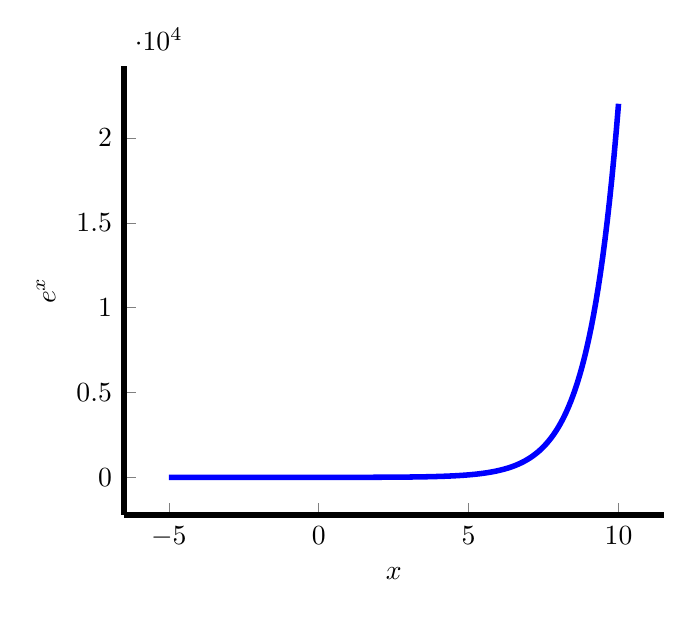
\begin{tikzpicture}
		\begin{axis}[every axis plot, line width=2pt,
				ylabel={$e^x$},
				xlabel={$x$},
				domain=-5:10,samples=200,
				axis x line*=bottom, % no box around the plot, only x and y axis
				axis y line*=left % the * suppresses the arrow tips
			]

			\addplot [blue] (x,{exp(x))});
		\end{axis}
	\end{tikzpicture}
\end{frame}

\subsection{Comparativo com a Regressão Linear}
\begin{frame}{Comparativo com a Regressão Linear}
	A regressão linear segue a seguinte formulação matemática:
	\small
	$$
		\text{Linear} = \alpha + \beta_1 x_1 + \beta_2 x_2 + \ldots + \beta_k x_k
	$$
	Onde:
	\begin{vfilleditems}
		\item \small $\alpha$ - constante
		\item \small $\boldsymbol{\beta} = \beta_1, \beta_2, \dots, \beta_k$ - coeficientes das variáveis independentes $x_1, x_2, \dots, x_k$
		\item \small $k$ - número de variáveis independentes
	\end{vfilleditems}
	Se você implementar uma pequena gambiarra matemática, você terá a \textbf{regressão de Poisson}:
	\begin{vfilleditems}
		\item \small $\log{y} = e^{\text{Linear}} = e^{\alpha + \beta_1 x_1 + \beta_2 x_2 + \ldots + \beta_k x_k}$
	\end{vfilleditems}
\end{frame}

\subsection{Especificação da Regressão de Poisson}
\begin{frame}{Especificação da Regressão de Poisson}
	Podemos fazer uma regressão de Poisson se a variável dependente
	$\boldsymbol{y}$ for uma variável com dados de contagem, ou seja,
	$\boldsymbol{y}$ somente toma valores positivos. A função de \textbf{verossimilhança de
		Poisson} usa uma constante $\alpha$ e os coeficientes $\boldsymbol{\beta}$
	porém estes são "exponenciados"~($e^x$):
	$$
		\begin{aligned}
			\boldsymbol{y}     & \sim \text{Poisson}\left( e^{(\alpha +  \mathbf{X} \boldsymbol{\beta})} \right) \\
			\alpha             & \sim \text{Normal}(\mu_\alpha, \sigma_\alpha)                                   \\
			\boldsymbol{\beta} & \sim \text{Normal}(\mu_{\boldsymbol{\beta}}, \sigma_{\boldsymbol{\beta}})
		\end{aligned}
	$$
\end{frame}

\subsection{Intepretação dos Coeficientes}
\begin{frame}{Interpretação dos Coeficientes}
	Ao vermos a fórmula de regressão de Poisson percebemos a interpretação dos
	coeficientes requer uma transformação. A transformação que precisamos fazer á a
	que inverte a função logarítmica:
	$$
		\log^{-1}(x) = e^x
	$$
	Então precisamos novamente "exponenciar"~os valores de $\alpha$ e
	$\boldsymbol{\beta}$:
	$$
		\begin{aligned}
			\boldsymbol{y} & = e^{(\alpha +  \mathbf{X} \boldsymbol{\beta})}                                                                                                                                         \\
			               & = e^{\alpha} \cdot e^{ \left( X_{(1)} \cdot \beta_{(1)} \right) } \cdot e^{ \left( X_{(2)} \cdot \beta_{(2)} \right) } \cdot \dots \cdot e^{ \left( X_{(k)} \cdot \beta_{(k)} \right) }
		\end{aligned}
	$$
\end{frame}

\subsection{Regressão de Poisson no \texttt{rstarnarm}}
\begin{frame}[fragile]{Regressão de Poisson no \href{http://mc-stan.org/rstanarm/}{\texttt{rstanarm}}}
	Usamos a função \texttt{stan\_glm()} com o argumento \texttt{poisson(link = "log")}:
	\vfill
	\begin{lstlisting}[basicstyle=\small]
    modelo_poisson <- stan_glm(
    y ~ ...,
    data = df,
    family = @poisson(link = "log")@,
    prior = ...,
    prior_intercept = ...
    )
    \end{lstlisting}
\end{frame}

\subsection{Regressão de Poisson no \texttt{brms}}
\begin{frame}[fragile]{Regressão de Poisson no \href{https://paul-buerkner.github.io/brms/}{\texttt{brms}}}
	Usamos a função \texttt{brm()} com o argumento \texttt{poisson(link = "log")}:
	\vfill
	\begin{lstlisting}[basicstyle=\small]
    modelo_poisson <- brm(
    y ~ ...,
    data = df,
    family = @poisson(link = "log")@,
    prior = c(
        set_prior("...", class = "b", coef = "..."),
                ...
        set_prior("...", class = "b", coef = "intercept")
        )
    )
    \end{lstlisting}
\end{frame}
